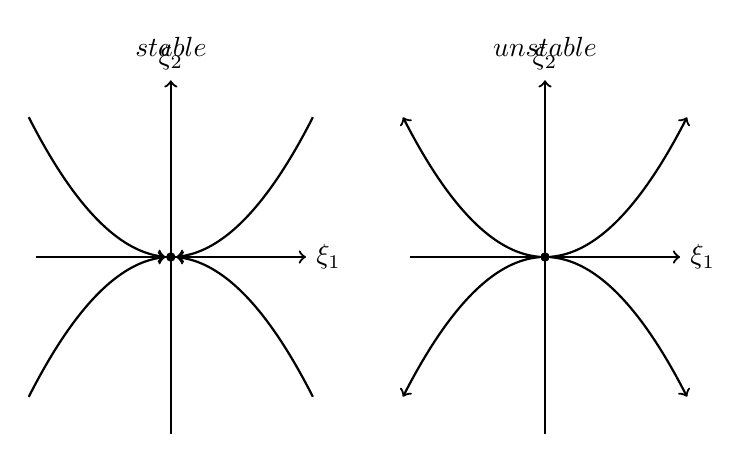
\begin{tikzpicture}[x=0.88cm,y=0.88cm,thick]
  \foreach \cx/\title in {-2.7/stable,2.7/unstable} {
    \draw[->] (\cx-1.95,0)--(\cx+1.95,0) node[right] {$\xi_1$};
    \draw[->] (\cx,-2.55)--(\cx,2.55) node[above] {$\xi_2$};
    \node[above] at (\cx,2.75) {$\title$};
    \fill (\cx,0) circle (1.7pt);
  }
  % Curves are tangent to the slow horizontal eigendirection at the node.
  \foreach \sgnx in {-1,1} {\foreach \sgny in {-1,1} {
    \draw[->] plot[domain=2.05:0.08,samples=65,variable=\s]
      ({-2.7+\sgnx*\s},{\sgny*0.48*\s*\s});
    \draw[->] plot[domain=0.08:2.05,samples=65,variable=\s]
      ({2.7+\sgnx*\s},{\sgny*0.48*\s*\s});
  }}
\end{tikzpicture}
